\section{Corpo nero}\label{sec:corpo-nero}

\subsection{Legge di Planck}\label{sec:legge-planck}
Introdotto da Planck alla fine del 1800, un \emph{corpo nero} è un corpo idealizzato in equilibrio termodinamico che assorbe tutta la radiazione incidente ed emette uno spettro che dipende solo dalla temperatura superficiale $T$ del corpo stesso. Il tasso di assorbimento e di emissione è lo stesso e la forma dello spettro del corpo segue la legge di Planck (fig.~\ref{fig:corpo-nero}):
\begin{equation}\label{eq:corpo-nero}
    B_{BB} (T) = \frac{2 h}{c^2} \frac{\nu^3}{e^{\frac{h \nu}{k_B T}} - 1}
\end{equation}
La planckiana dipende sia dalla \emph{frequenza} che dalla \emph{temperatura} del corpo. Le stelle in prima approssimazione si possono considerare dei corpi neri, come si può osservare da un confronto tra dati sperimentali e curve teoriche in fig.~\ref{fig:stelle-corpi-neri}. Guardando come sono fatte le curve a diverse lunghezze d'onda si può inferire la \emph{legge di spostamento di Wien}.

\begin{figure}
\centering
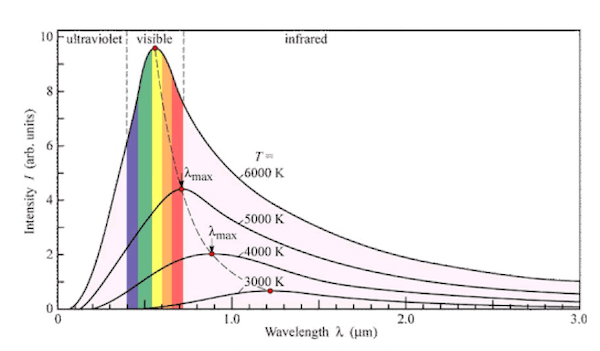
\includegraphics[width=0.5\textwidth]{immagini/corpo-nero.png}
\caption{Legge di Planck. Curve in funzione della frequenza plottate a diverse temperature. I picchi seguono la legge di spostamento di Wien.}
\label{fig:corpo-nero}
\end{figure}

\begin{figure}
\centering
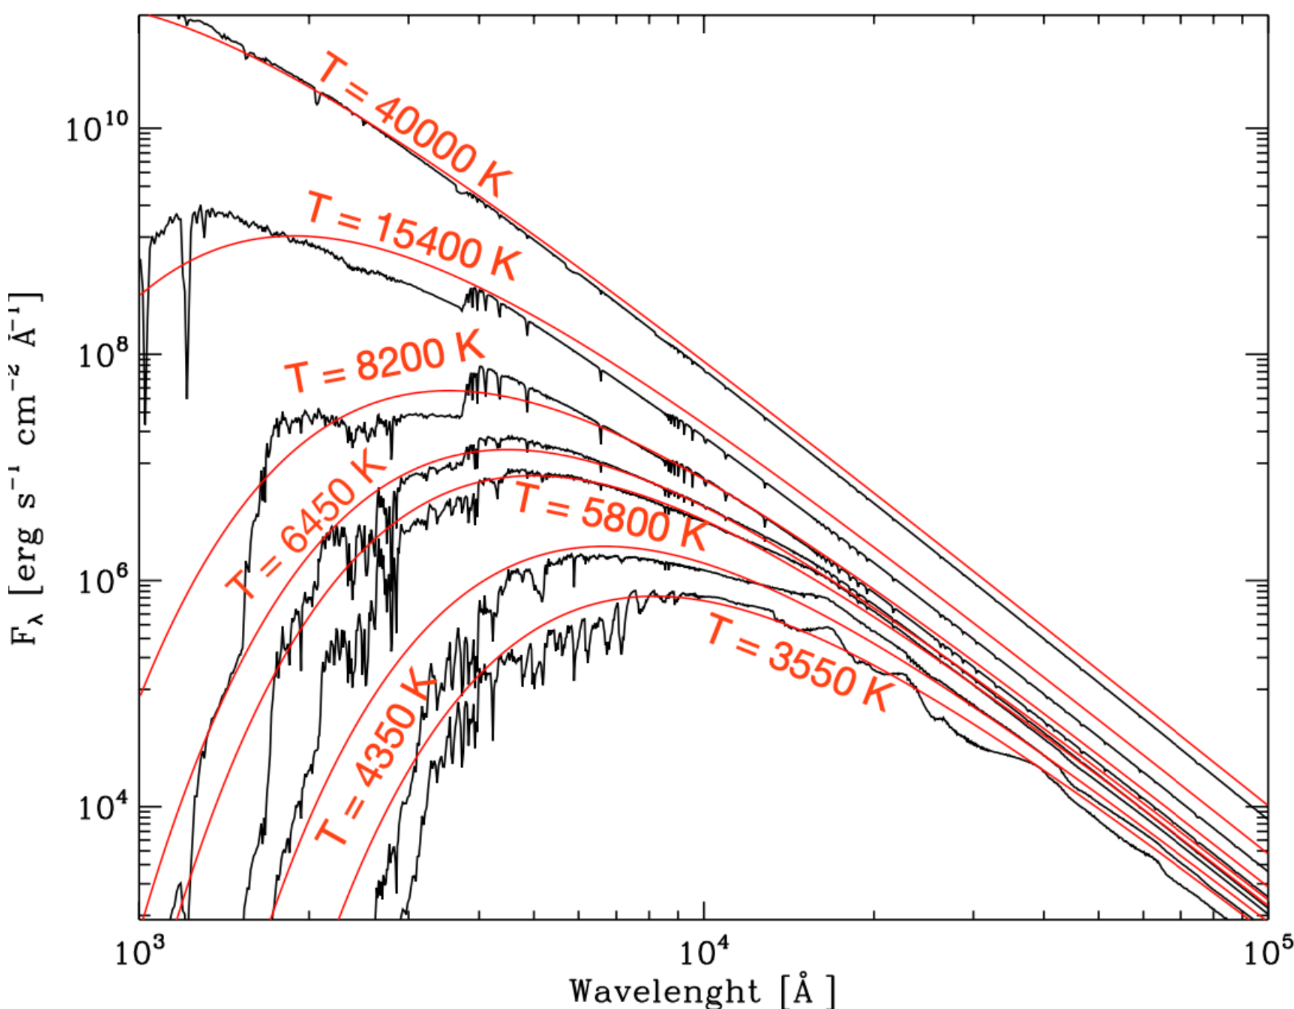
\includegraphics[width=0.4\textwidth]{immagini/stelle-corpi-neri.png}
\caption{Confronto tra i profili teorici di planckiana e dati sperimentali delle stelle. In prima approssimazione le stelle possono essere trattate come corpi neri.}
\label{fig:stelle-corpi-neri}
\end{figure}

\subsection{Legge di spostamento di Wien}\label{sec:legge-wien}
Più elevata è la temperatura $T$ del corpo, più il picco di emissione si trova a basse lunghezze d'onda, corrispondenti ad alte frequenze (fig.~\ref{fig:corpo-nero}):
\begin{equation}\label{eq:legge-wien}
    T \lambda_\textup{max} = \SI{0.29}{cm.K}
\end{equation}
Da questa legge è immediato capire perché vediamo il nostro sole di colore giallo. Infatti, la sua temperatura superficiale è circa $T \sim \SI{5770}{K}$, da cui una lunghezza d'onda sul picco corrispondente a $\lambda_\textup{max} \sim \SI{0.5}{\mu m}$. Si può esprimere la legge di Wien anche in funzione della frequenza, come mostrato in fig.~\ref{fig:legge-wien}. Si nota che più elevata è la temperatura del corpo, più il picco di emissione si trova ad alte frequenze (basse lunghezze d'onda). Dunque, supponendo che una sorgente osservata sia un corpo nero ed effettuando misure a diverse frequenze (lunghezze d'onda), in base alla frequenza (lunghezza d'onda) a cui si osserva il picco di emissione è possibile risalire alla temperatura superficiale della stella. In particolare, una \emph{stella blu} sarà \emph{calda}, mentre una \emph{stella rossa} sarà \emph{fredda}.

\begin{figure}
\centering
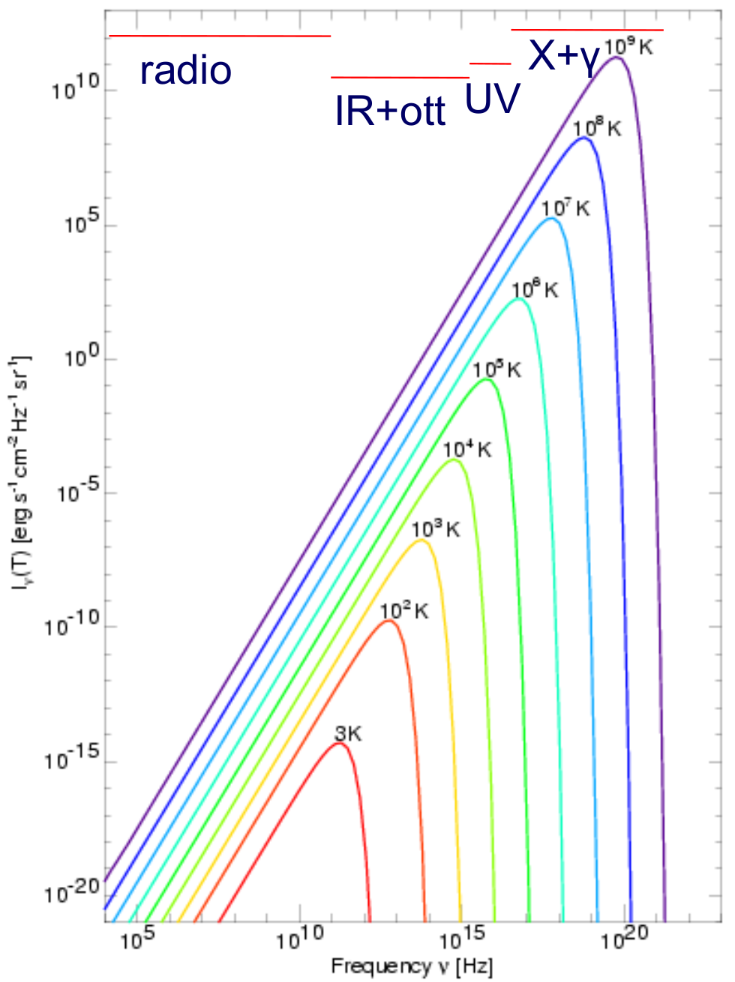
\includegraphics[width=0.3\textwidth]{immagini/legge-wien.png}
\caption{Legge di Wien vista in funzione della frequenza. All'aumentare della temperatura, il picco di emissione si sposta verso frequenze più alte.}
\label{fig:legge-wien}
\end{figure}

\subsection{Legge di Stefan-Boltzmann}\label{sec:legge-stefan-boltzmann}
Osservando lo spettro di corpo nero, eq.~\eqref{eq:corpo-nero}, è possibile inferire che debba esserci una relazione tra la temperatura $T$ e la luminosità bolometrica di una stella, $L_\textup{bol}$. Infatti, all'aumentare di $T$ aumenta l'intensità del corpo nero (l'energia emessa per unità di tempo), ovvero, integrando su tutte le lunghezze d'onda, aumenta l'area sottesa dalla curva~\ref{fig:corpo-nero}. La luminosità integrata su tutte le frequenze è proprio la luminosità bolometrica (si veda par.~\ref{sec:luminosità} ed eq.~\eqref{eq:def-luminosità-bolometrica} e~\eqref{eq:luminosità-bolometrica}).

Gli esperimenti di \emph{Josef Stefan} (1879) hanno mostrato che la luminosità bolometrica $L_\textup{bol}$ di un corpo nero di area $A$ alla temperatura $T$, misurata in Kelvin, è data da:
\[
    L_\textup{bol} = A \sigma T^4
\]
dove $\sigma$ è la \emph{costante di Stefan-Boltzmann} e vale:
\[
    \sigma = \SI{5.67e-5}{erg.s^{-1}.cm^{-2}.K^{-4}}
\]
Dunque, data una stella di raggio $R$ e \emph{temperatura superficiale} T:
\begin{equation}\label{eq:stefan-boltzmann}
    L_\textup{bol} = 4 \pi R^2 \sigma T^4
\end{equation}
Inserendo i dati del Sole
\[
    R \sim \SI{7e10}{cm} \qquad T \sim \SI{5770}{K}
\]
si ottiene
\[
    \si{\solarluminosity} \sim \SI{3.8e-33}{erg.s^{-1}}
\]
Si può utilizzare la legge~\eqref{eq:stefan-boltzmann}, ad esempio, per ricavare il raggio di una stella, conoscendone la temperatura superficiale e la luminosità, posto che l'ipotesi di corpo nero sia accurata.